\documentclass[letterpaper, 12pt]{article}

\usepackage[utf8]{inputenc}
\usepackage[english, spanish]{babel}
\usepackage{fullpage}
\usepackage{graphicx}
\usepackage{amsmath}
\usepackage{enumitem}
\usepackage{chngcntr}
\usepackage{setspace}
\usepackage{url}
\usepackage{csquotes}
\usepackage{float}
\usepackage{verbatim}
\usepackage{tabularx}
\usepackage{amsmath}
\usepackage{caption}
\usepackage{bm}
\usepackage{colortbl}
\usepackage{xcolor}

\usepackage{multirow}

% \usepackage{hyperref}

\counterwithin{figure}{section}
\renewcommand{\thesection}{\arabic{section}}
\renewcommand{\thesubsection}{\thesection.\arabic{subsection}}
\renewcommand{\baselinestretch}{1.5}

\usepackage[style=numeric, maxnames=6, minnames=3, backend=biber, parentracker=true, sorting=none]{biblatex}
\DefineBibliographyStrings{english}{%chktex-file 1 chktex-file 6
      andothers = {\em et\addabbrvspace al\adddot}
}
\addbibresource{./Bibliography/bibliography.bib}

\usepackage{array}

\setlength{\parskip}{0pt}

\raggedbottom{}

\newcommand{\bolditalic}[1]{\textbf{\textit{#1}}}

\newcommand{\Celsius}[0]{°$\mathcal{C}$}
\newcommand{\Kelvin}[0]{$\mathcal{K}$}
\newcommand{\Fahrenheit}[0]{°$\mathcal{F}$}

\begin{document}

\begin{titlepage}
      \centering
      
\includegraphics[width=0.3\textwidth]{Images/logo_utb.png}\par\vspace{1cm}
      {\scshape\LARGE Universidad Tecnológica de Bolívar \par}
      \vspace{1cm}

      {\scshape\Large FÍSICA CALOR Y ONDAS \par}
      \vspace{.2cm}

      % chktex-file 8
      {\scshape\Large Grupo 1 \par}
      \vspace{1cm}
      % chktex-file 8
      \slshape {\Large \bfseries{}Informe de Laboratorio No. V\\}
      \slshape {\small \bfseries{}CALOR ESPECÍFICO DE LOS SÓLIDOS}
      \vspace{2cm}

      \slshape {\itshape{} Mauro González, T00067622 \\}
      \slshape {\itshape{} German De Armas Castaño, T00068765 \\}
      \slshape {\itshape{} Angel Vega Rodriguez, T00068186 \\}
      \slshape {\itshape{} Juan Jose Osorio Ariza, T00067316 \\}
      \slshape {\itshape{} Jorge Alberto Rueda Salgado, T00068722 \\}
      \vfill
      Revisado Por \\
      Duban Andres Paternina Verona\\
      {\large \today\par}
\end{titlepage}

% chktex-file 44
% chktex-file 24

% ! ----------------------------------------------------------------------|>
\section{Introducción}

La determinación del calor específico de los sólidos es una
parte fundamental de la termodinámica y juega un papel
esencial en la comprensión de cómo los materiales almacenan
y liberan energía térmica. En esta experiencia de
laboratorio, se lleva a cabo un estudio detallado de la
transferencia de calor entre sólidos y líquidos para
determinar el calor específico de varios materiales. Esto
se logra mediante la medición de cambios de temperatura y
la aplicación de principios termodinámicos fundamentales.
La experimentación práctica en esta área es crucial para la
aplicación de conceptos teóricos en situaciones del mundo
real y es esencial para una amplia gama de campos, desde la
física hasta la ingeniería.

% ! ----------------------------------------------------------------------|>
\section{Objetivos}

% + ----------------------------------------|>
\subsection{Objetivo general}

El objetivo principal de esta práctica de laboratorio es
determinar el calor específico de sólidos utilizando un
enfoque experimental basado en la transferencia de calor y
principios termodinámicos.

% + ----------------------------------------|>
\subsection{Objetivos específicos}

\begin{itemize}[label=$\triangleright$]
      \item Medir la temperatura inicial y final de una mezcla de agua
            y sólidos después de una transferencia de calor controlada.

      \item Determinar la masa equivalente del calorímetro utilizado en
            el experimento.

      \item Calcular el calor específico de los sólidos utilizando los
            datos recopilados y las ecuaciones pertinentes.

      \item Comparar los resultados obtenidos utilizando dos métodos
            diferentes para calcular el calor específico.
\end{itemize}

% ! ----------------------------------------------------------------------|>
\section{Marco Teórico}

% + -------------------------------------------------------------|>
\subsection{Calor}

El calor se refiere a la transferencia de energía térmica
entre dos sistemas que están a diferentes temperaturas.
Esta transferencia de energía se produce debido a la
diferencia de temperatura entre los sistemas y ocurre
siempre desde el sistema de mayor temperatura hacia el
sistema de menor temperatura.

Es importante destacar que el calor es una forma de energía
en tránsito y no una propiedad intrínseca de un objeto o
sustancia en sí misma. Se puede medir en unidades de
energía, como calorías (en el sistema métrico) o BTUs (en
el sistema imperial).

Existen tres formas comunes de transferir calor:

\begin{enumerate}
      \item Conducción: Es la transferencia de calor a través de
            materiales que están en contacto directo. En este proceso,
            las partículas de un material transfieren su energía
            térmica a las partículas adyacentes.

      \item Convección: Se refiere a la transferencia de calor en
            fluidos (líquidos y gases) debido a la circulación de las
            partículas del fluido. Esto sucede cuando una corriente de
            fluido caliente asciende y una corriente de fluido frío
            desciende.

      \item Radiación: Es la transferencia de calor a través de ondas
            electromagnéticas, como la luz o el calor que sentimos del
            sol. Esta forma de transferencia de calor no requiere un
            medio material y puede ocurrir incluso en el vacío.
\end{enumerate}

% + -------------------------------------------------------------|>
\subsection{Temperatura}

La temperatura es una medida de la energía cinética
promedio de las partículas en un sistema. En términos más
simples, indica cuán caliente o frío está un objeto o una
sustancia. Cuando decimos que algo tiene una alta
temperatura, significa que las partículas que lo componen
están vibrando o moviéndose rápidamente, mientras que una
baja temperatura indica que las partículas están más
tranquilas y tienen menos energía cinética.

% * --------------------------------------------------------|>
\subsubsection{Escalas de temperatura}

Las escalas de temperatura son sistemas de medición que se
utilizan para cuantificar y comparar temperaturas. Existen
varias escalas de temperatura en uso en todo el mundo, pero
las tres más comunes son Celsius (\Celsius), Fahrenheit
(\Fahrenheit) y Kelvin (\Kelvin). Cada una tiene su propia
base y forma de referencia.

\begin{itemize}[label=$\triangleright$]
      \item Celsius (\Celsius): También conocida como escala
            centígrada, la escala Celsius se basa en los puntos de
            congelación y ebullición del agua a una presión atmosférica
            normal. En esta escala, el punto de congelación del agua se
            establece en 0 grados Celsius y el punto de ebullición se
            establece en 100 grados Celsius. Es la escala de
            temperatura más comúnmente utilizada en todo el mundo para
            propósitos cotidianos.

      \item Fahrenheit (\Fahrenheit): Esta escala fue desarrollada por
            el físico Daniel Gabriel Fahrenheit. Se basa en puntos de
            referencia relacionados con el clima y utiliza el punto de
            congelación del agua mezclada con sal y el punto de
            ebullición del agua pura para establecer sus puntos de
            referencia. En la escala Fahrenheit, el punto de
            congelación del agua se ubica en 32 grados Fahrenheit y el
            punto de ebullición en 212 grados Fahrenheit. Esta escala
            se utiliza principalmente en los Estados Unidos y en
            algunos otros países.

      \item Kelvin (\Kelvin): La escala Kelvin es una escala de
            temperatura absoluta basada en cero absoluto, que es la
            temperatura más baja posible. En esta escala, el cero
            absoluto se sitúa en 0 Kelvin y representa la completa
            ausencia de energía térmica. Las temperaturas en la escala
            Kelvin se utilizan principalmente en la ciencia y la
            ingeniería, especialmente en áreas como la física, la
            química y la astronomía.
\end{itemize}

Es importante destacar que la relación entre las diferentes
escalas de temperatura es lineal. Es decir, un cambio de 1
grado en la escala Celsius es equivalente a un cambio de 1
grado en la escala Kelvin, pero no es equivalente a un
cambio de 1 grado en la escala Fahrenheit.

% + -------------------------------------------------------------|>
\subsection{Ley cero de la termodinámica}

Establece el concepto de equilibrio térmico y proporciona
la base para la definición precisa de temperatura. Esta ley
afirma: ``Si dos sistemas están en equilibrio térmico con
un tercer sistema, entonces están en equilibrio térmico
entre sí''.

En otras palabras, si dos cuerpos están en equilibrio
térmico con un tercer cuerpo, entonces están también en
equilibrio térmico entre sí, lo que significa que no habrá
intercambio neto de calor entre ellos.

Esta ley es fundamental porque establece una base para
definir y medir la temperatura. Si dos sistemas están en
equilibrio térmico, sus temperaturas son iguales. Esto
proporciona una manera precisa de comparar y medir
temperaturas, lo que es crucial en todos los aspectos de la
termodinámica.

La Ley Cero también es la razón por la cual se utilizan
termómetros para medir la temperatura. Un termómetro
funciona tomando ventaja de la expansión o contracción de
una sustancia (como el mercurio en un termómetro de
mercurio) con cambios de temperatura. Cuando el sistema de
medición (el termómetro) alcanza el equilibrio térmico con
el sistema que se está midiendo, la lectura del termómetro
proporciona una medida precisa de la temperatura del
sistema.

% + -------------------------------------------------------------|>
\subsection{Primera ley de la termodinámica}

También conocida como el principio de conservación de la
energía para procesos termodinámicos, establece que la
energía total en un sistema aislado se mantiene constante.
En términos más simples, la energía no puede ser creada ni
destruida, solo transformada de una forma a otra.
Matemáticamente, la Primera Ley se expresa como:

\begin{equation*}
      \Delta U = Q - W
\end{equation*}

\begin{itemize}[label=$\triangleright$]
      \item $\Delta U$ representa el cambio en la energía interna del sistema.
      \item $Q$ es la cantidad de calor añadida al sistema.
      \item $W$ es el trabajo realizado por el sistema.
\end{itemize}

Es importante notar que la Primera Ley de la Termodinámica
se aplica a sistemas cerrados, es decir, sistemas que no
intercambian materia con su entorno, pero sí pueden
intercambiar energía en forma de calor y trabajo.

% + -------------------------------------------------------------|>
\subsection{Calor especifico}

El calor específico de una sustancia es una propiedad
física que indica la cantidad de calor que se necesita para
elevar la temperatura de una unidad de masa de esa
sustancia en una cantidad específica. En otras palabras, es
la cantidad de energía térmica que se debe agregar o quitar
a una sustancia para cambiar su temperatura en una unidad
de masa en una cierta cantidad.

Matemáticamente, el calor específico (C) se define como:

\begin{equation*}
      C = \frac{q}{m \cdot \Delta T}
\end{equation*}

Donde,

\begin{itemize}
      \item $C$ es el calor específico de la sustancia.
      \item $q$ es la cantidad de calor agregada o quitada.
      \item $m$ es la masa de la sustancia.
      \item $\Delta T$ es el cambio en la temperatura.
\end{itemize}

% + -------------------------------------------------------------|>
\subsection{Energía cinética}

Es una forma de energía asociada al movimiento de un
objeto. Se define como la energía que un objeto posee
debido a su velocidad y masa. La fórmula para calcular la
energía cinética (EC) es la siguiente:

\begin{equation*}
      EC = \frac{1}{2} \cdot m v^{2}
\end{equation*}

Donde,

\begin{itemize}
      \item $m$ es la masa del objeto en movimiento.
      \item $v$ es la velocidad del objeto.
\end{itemize}

Esta fórmula nos dice que la energía cinética es
directamente proporcional al cuadrado de la velocidad del
objeto y a su masa. Esto significa que un objeto con mayor
masa o velocidad tendrá una mayor energía cinética.

% ! ----------------------------------------------------------------------|>
\section{Montaje Experimental}

\begin{figure}[H]
      \begin{center}
            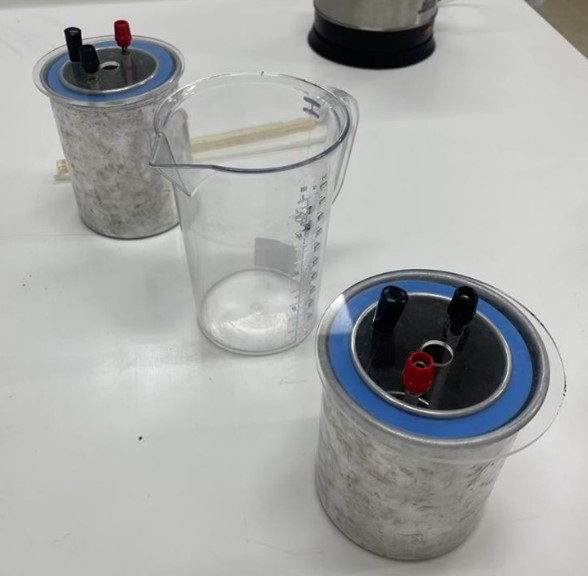
\includegraphics[width=.5\linewidth]{./Images/Montaje1.jpg}
            \caption{}
      \end{center}
\end{figure}

\begin{figure}[H]
      \begin{center}
            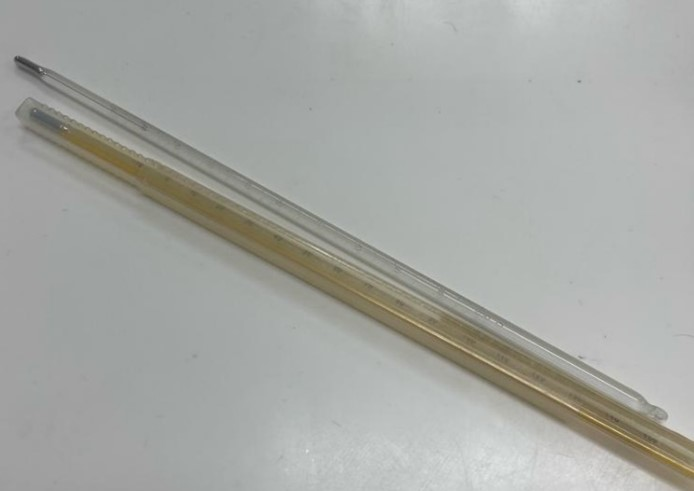
\includegraphics[width=.5\linewidth]{./Images/Montaje2.jpg}
            \caption{}
      \end{center}
\end{figure}

\begin{figure}[H]
      \begin{center}
            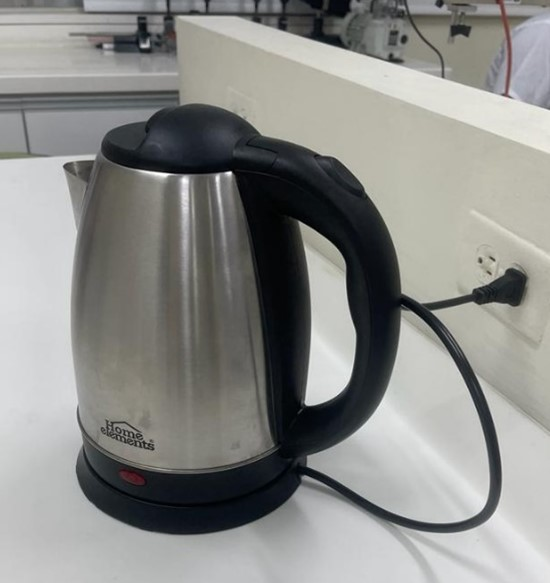
\includegraphics[width=.5\linewidth]{./Images/Montaje3.jpg}
            \caption{}
      \end{center}
\end{figure}

\begin{figure}[H]
      \begin{center}
            
\includegraphics[width=.5\linewidth]{./Images/Montaje4.jpg}
            \caption{}
      \end{center}
\end{figure}

Equipo utilizado:

\begin{itemize}
      \item Vaso de Dewar con tapa (calorímetro).

      \item Bloque o gránulos de cobre, aluminio o Hierro.

      \item Termómetro –10 C a +110 °C o sensor de temperatura NiCr-Ni.

      \item Generador de vapor, 550 W / 220 V.

      \item Aparatos de calefacción.

      \item Vaso de precipitados, 400 -600 ml
\end{itemize}

% ! ----------------------------------------------------------------------|>
\section{Datos Experimentales}

En esta experiencia realizamos un proceso para determinar
el equivalente en agua del calorímetro $m_k$ y el calor
específico de sólidos. Primero, se mezcló agua en el
calorímetro y se midió su temperatura inicial. Luego, se
añadió agua calentada al calorímetro y se registró la
temperatura de equilibrio. Para el calor específico de
sólidos, se midió la masa del sólido, se calentó con agua y
se registraron temperaturas. Luego, se transfirió el sólido
al calorímetro y se monitoreó la temperatura.
Permitiéndonos obtener los siguientes resultados.

\begin{table}[H]
      \begin{center}
            \begin{tabularx}{.9\linewidth}{|>{\centering\arraybackslash}X|>{\centering\arraybackslash}X|>{\centering\arraybackslash}X|>{\centering\arraybackslash}X|}
                  \hline
                  \multirow{3}{*}{Cuerpo} & \multirow{3}{*}{Masa (Kg)} & Temperaturas iniciales $T_0$ Y T~(\Celsius) & Temperatura final $T_e$~(\Celsius) \\\hline

                  M                       & 0,25                       & 28                                          & 40                                 \\\hline

                  m                       & 0,08                       & 92                                          & 40                                 \\\hline
            \end{tabularx}
      \end{center}
\end{table}

\begin{table}[H]
      \begin{center}
            \begin{tabularx}{.9\linewidth}{|>{\centering\arraybackslash}X|>{\centering\arraybackslash}X|>{\centering\arraybackslash}X|>{\centering\arraybackslash}X|}
                  \hline
                  Sustancia   & Masa (Kg) & $T_0$\Celsius & $T_m$ de equilibrio \\\hline

                  Calorímetro & 0,25      & \dots         & 31                  \\\hline

                  Agua        & 0.2       & 28            & 31                  \\\hline

                  Solido      & 0,0964    & 91            & 31                  \\\hline
            \end{tabularx}
      \end{center}
\end{table}

% ! ----------------------------------------------------------------------|>
\section{Análisis de datos}

% + -------------------------------------------------------------|>
\subsection{Análisis}

% * --------------------------------------------------------|>
\subsubsection{}

Ecuación 2:~$Q_1 = C_1 m_1 (T_1 - T_M)$, Ecuación 3:~$Q_2 =
      C_2 m_2 (T_2 - T_M)$, Ecuación 4:~$Q_1 + Q_2$

Reemplazando (2) y (3) en (4), obtenemos,

$C_1 m_1 (T_1 - T_M) + C_2 m_2 (T_2 - T_M) = 0$

Luego se despeja $C_1$

\begin{equation*}
      \begin{gathered}
            C_1 m_1 (T_1 - T_M) = -C_2 m_2 (T_2 - T_M) \\
            C_1 = \frac{- C_2 m_2 (T_2 - T_M)}{m_1 (T_1 - T_M)} \\
            C_1 = C_2 \frac{m_2 (T_M - T_2)}{m_1 (T_1 - T_M)}~\surd
      \end{gathered}
\end{equation*}

% * --------------------------------------------------------|>
\subsubsection{}

Ecuación 7:~$Q_2 = C_2 (m_2 + m_k)(T_M - T_2)$, Ecuación
2:~$Q_1 = C_1 m_1 (T_1 - T_M)$, Ecuación 4:~$Q_1 + Q_2 = 0$

Reemplazando (2) y (7) en (4)

$C_2 (m_2 + m_k)(T_M T_2) + C_1 m_1 (T_1 - T_M) = 0$

Luego se despeja $C_1$ de la ecuación

\begin{equation*}
      \begin{gathered}
            C_1 = \frac{- C_2(m_2 + m_k)(T_M - T_2)}{m_1 (T_1 - T_M)} \\
            C_1 = C_2 \frac{(m_2 + m_k)(T_M - T_2)}{m_1 (T_1 - T_M)}~\surd
      \end{gathered}
\end{equation*}

% * --------------------------------------------------------|>
\subsubsection{}

Ecuación 10:~$m_K = \frac{m (T - T_e)}{T_e - T_o}$

Reemplazando los valores, $m_K = \frac{0.08 (92 - 40)}{40 -
            28} = 0.097 Kg$

% * --------------------------------------------------------|>
\subsubsection{}

Utilizando la ecuación,

\begin{equation}
      C_{1} = C_{2} \frac{m_{2} (T_{m} - T_{2})}{m_1 (T_{1} - T_{m})}
      \label{eq:calor_especifico_1}
\end{equation}

Donde,

\begin{itemize}[label=$\triangleright$]
      \item $m_{1}$: masa del sólido,
      \item $C_{1}$: su calor especifico
      \item $m_{2}$: masa del agua,
      \item $C_{2}$: el calor específico de calor del agua,
      \item $T_{1}$: temperatura de la sustancia,
      \item $T_{2}$: temperatura del agua,
      \item $T_{m}$: temperatura común.
\end{itemize}

El calor específico del agua es de: \hfill{} \break{}
$C_{2} = 4.19\frac{J}{K\cdot KG}$

\smallskip

Conversiones:

\begin{itemize}[label=$\triangleright$]
      \item $m_{1}$: $96.4$~g = $0.0964$~kg
      \item $m_{2}$: $200$~g = $0.20$~kg
      \item $T_{m}$: $31$\Celsius = $304.15$~\Kelvin
      \item $T_{1}$: $91$\Celsius = $364.15$~\Kelvin
      \item $T_{2}$: $28$\Celsius = $301.15$~\Kelvin
\end{itemize}

\begin{equation*}
      \begin{gathered}
            C_{1} = 4.19 \frac{J}{K \cdot Kg} \times \frac{0.20 Kg (304.15~\mathcal{K} - 301.15~\mathcal{K})}{0,0964 Kg(364.15~\mathcal{K} - 304.15~\mathcal{K})} \\
            C_{1} = 0.435 \frac{J}{K \cdot Kg}
      \end{gathered}
\end{equation*}

% * --------------------------------------------------------|>
\subsubsection{}

\begin{equation}
      C_{1} = C_{2} \frac{(m_{2} + m_{k})(T_{M} - T_{2})}{m_{1}(T_{1} - T_{M})}
      \label{eq:calor_especifico_2}
\end{equation}

Masa del calorímetro:

\begin{equation}
      m_{k} = \frac{m(T - T_{e})}{T_{e} - T_{0}} - M
      \label{eq:masa_calorimetro}
\end{equation}

Donde,

\begin{itemize}[label=$\triangleright$]
      \item $T_{0}$: temperatura del agua en el calorímetro sin calentar
      \item $T$: temperatura del agua calentada
      \item $T_{e}$: temperatura en equilibrio
      \item $M$: gramos de agua iniciales
      \item $m$: gramos de agua añadidos
\end{itemize}

Conversiones:

\begin{itemize}
      \item $M$: $250$g = $0.25$~Kg
      \item $m$: $80$g = $0.08$~Kg
      \item $T_{0}$: $28$\Celsius = $301.15$~\Kelvin
      \item $T$: $92$\Celsius = $365.15$~\Kelvin
      \item $T_{e}$: $40$\Celsius = $313.15$~\Kelvin
\end{itemize}

\begin{equation*}
      \begin{gathered}
            m_k = \frac{0,08 Kg(365.15~\mathcal{K} - 313.15~\mathcal{K})}{313.15~\mathcal{K} - 301.15~\mathcal{K}} \\
            m_k = 0.097 Kg
      \end{gathered}
\end{equation*}

\begin{equation*}
      \begin{gathered}
            C_{1} = 4.19 \frac{J}{K \cdot Kg} \times \frac{(0.020 Kg + 0.097 Kg)(304.15~\mathcal{K} - 301.15~\mathcal{K})}{0,0964 Kg(364.15~\mathcal{K} - 304.15~\mathcal{K})} \\
            C_{1} = 0.645 \frac{J}{K \cdot Kg}
      \end{gathered}
\end{equation*}

% * --------------------------------------------------------|>
\subsubsection{}

\begin{itemize}[label=$\triangleright$]
      \item En el punto 4, se calculó el calor específico ($C_1$)
            utilizando la ecuación (\ref{eq:calor_especifico_1}).\@{}El
            valor obtenido fue aproximadamente $0.435 \frac{J}{K \cdot
                        Kg}$.

      \item En el punto 5, se volvió a calcular el calor específico
            ($C_1$) utilizando la ecuación
            (\ref{eq:calor_especifico_2}), teniendo en cuenta la masa
            del calorímetro. El valor obtenido fue aproximadamente
            $0.435 \frac{J}{K \cdot Kg}$.

            En el punto 5, se considera la masa del calorímetro, que es
            de $0.25$ kg. El calorímetro es la parte del sistema que
            almacena el calor y, por lo tanto, afecta la cantidad de
            calor que puede absorber o liberar durante un cambio de
            temperatura. Cuando se calcula el calor específico (C1)
            utilizando la ecuación HERE, la masa total del sistema
            ($m_2$ + $m_k$) en el denominador es la suma de la masa del
            calorímetro ($m_k$) y la masa de agua añadida ($m_2$). Esto
            significa que el calorímetro en sí mismo contribuye a la
            capacidad térmica total del sistema. Por lo tanto, el
            resultado de C1 se ve influenciado por la masa del
            calorímetro y cómo esta afecta la absorción de calor
            durante el experimento.

            En resumen, los dos métodos utilizados para determinar el
            calor específico
            (\ref{eq:calor_especifico_1})~(\ref{eq:calor_especifico_2})
            proporcionaron resultados ligeramente diferentes. Esto
            puede deberse a las diferencias en las ecuaciones y a la
            consideración de la masa del calorímetro en el punto 5.
            Considerar la masa del calorímetro es crucial, ya que
            afecta directamente el resultado final del cálculo del
            calor específico ($C_1$). La masa del calorímetro se suma a
            la masa total del sistema y contribuye a su capacidad
            térmica, lo que hace que el resultado de $C_1$ sea más
            preciso y realista en condiciones experimentales.
\end{itemize}

% ! ----------------------------------------------------------------------|>
\section{Conclusiones}

En esta experiencia de laboratorio, se llevaron a cabo
mediciones precisas de la transferencia de calor entre
sólidos y agua. Se determinaron los calores específicos de
los sólidos utilizando dos métodos diferentes, uno que
considera el calor absorbido por el agua y otro que tiene
en cuenta la masa equivalente del calorímetro. Se
encontraron diferencias en los resultados obtenidos por
estos métodos, lo que demuestra la importancia de
considerar la contribución del calorímetro en el proceso.

Estos experimentos proporcionaron una comprensión práctica
de los conceptos fundamentales de la termodinámica y
demostraron la relación entre la masa, la temperatura y el
calor específico de los sólidos. Además, destacaron la
necesidad de la precisión en la medición y la importancia
de la calibración adecuada de los instrumentos utilizados
en experimentos de transferencia de calor.

\printbibliography

\end{document}